\section{Auswertung}

Bevor wir das SQUID eingeschaltet haben, haben wir noch die Distanz der Probe zum SQUID-Sensor gemessen. Diese beträgt:

$$z = (3,6 \pm 0,2)\ cm$$

Nach dieser Messung haben wir den flüssigen Stickstoff in das Kryostat gefüllt und den SQUID-Sensor eingefügt. Wir haben 15 Minuten gewartet, und dann mit der Justierung begonnen.

\subsection{Justierung des SQUIDs}

Die Justierung des SQUIDs haben wir anhand des Programms \emph{JSQ Duo Sensor Control} an einem PC und einem Oszilloskop durchgeführt. Wir haben die Software in den Test-Modus geschaltet, welcher einen Funktionsgenerator dazu veranlasst, eine Dreieckspannung in den Schwingkreis einzukoppeln. Diese beeinflusst dann die Spannungsantwort des SQUID, die wir am Oszilloskop einsehen können, das sogenannte \emph{SQUID-Pattern}. Zum Triggern schließen wir dann den Funktionsgenerator noch direkt an den Oszilloskop.  Dann haben wir den Arbeitspunkt anhand der Software justiert, sodass die Amplitude des SQUID-Patterns maximal wurde. Unsere Einstellparameter lauten:\\

\centering \begin{tabular}[H]{l l}
	$VCA = 1391$ & Stromamplitude des Schwingkreises ($\sim 6\cdot 10^{-8} W$)\\
	$VCO = 1477$ & Frequenz des Schwingkreises ($\sim 760 MHz$)\\
	$OFF = 1471$  & Offset des Signals
\end{tabular}

%\begin{figure}[H]
%	\centering 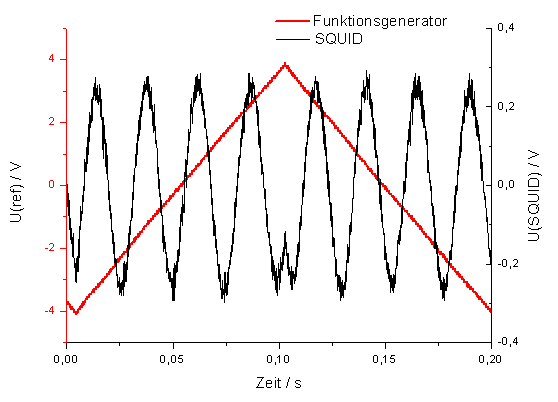
\includegraphics[width = \textwidth]{Bilder/Pattern1.jpg}
%	\caption{Das SQUID-Pattern}
%\end{figure}

\subsection{Leiterschleife}

Wir haben eine stromdurchflossene Leiterschleife mit Durchmesser $d = (3,5 \pm 0,3)\ mm$ am SQUID für 5 verscheide Widerstände gemessen:\\


\begin{tabular}[H]{c | c}
	Widerstand & Spannungsabfall\\ \hline \hline
	$R_1 = (51,3 \pm 0,1)\ \Omega$ & $U_1 = (2,11 \pm 0,01) \ V$ \\
	$R_2 = (101,3 \pm 0,1)\ \Omega$ & $U_2 = (2,51 \pm 0,01) \ V$ \\
	$R_3 = (302 \pm 1)\ \Omega$ & $U_3 = (2,75 \pm 0,01) \ V$ \\
	$R_4 = (513 \pm 1)\ \Omega$ & $U_4 = (2,82 \pm 0,01) \ V$ \\
	$R_5 = (1008 \pm 1)\ \Omega$ & $U_5 = (2,87 \pm 0,01) \ V$
\end{tabular}
